%% ----------------------------------------------------------------
%% PACKAGES
%% ----------------------------------------------------------------
\documentclass[titlepage, 12pt]{article}
\usepackage[table, xcdraw, dvipsnames]{xcolor}
\usepackage[utf8]{inputenc}
\usepackage[spanish]{babel}
\usepackage{amsmath}
\usepackage{booktabs}
\usepackage[RPvoltages]{circuitikz}
\usepackage{enumitem}
\usepackage{fancyhdr}
\usepackage{float}
\usepackage{geometry}
\usepackage{graphicx}
\usepackage[hidelinks]{hyperref}
\usepackage{lastpage}
\usepackage{pdflscape}
\usepackage{parskip}
\usepackage{siunitx}
\usepackage{subcaption}
\usepackage{tabularx}
\usepackage{tabulary}
\usepackage{tikz}
\usepackage{xfrac}
\usepackage{layouts}

%% ----------------------------------------------------------------
%% SETTINGS
%% ----------------------------------------------------------------
\decimalpoint
\geometry{
  a4paper,
  total={170mm,247mm},   %210x297mm
  left=20mm,
  top=20mm,
}
\renewcommand{\tablename}{Tabla}
\newcommand{\fecha}{14/08/2021}
\newcommand{\version}{3.0}


%% ----------------------------------------------------------------
%% HEADER/FOOTER
%% ----------------------------------------------------------------
\pagestyle{fancy}
\fancyhf{}
\lhead{Calibrador y caracterizador de sondas de corriente}
\rhead{Especificación de requerimientos}
\lfoot{Fecha: \fecha}
\cfoot{Versión \version}
\rfoot{Página \thepage \hspace{1pt} de \pageref{LastPage}}

\setlength{\headheight}{30pt}


%% ----------------------------------------------------------------
%% TITLE
%% ----------------------------------------------------------------
\title{Especificación de requerimientos:\\Calibrador y caracterizador de sondas de corriente}
\author{Agustín Aon Sanchez\\
Facultad de Ingeniería\\
Universidad Nacional de Mar del Plata}
\date{Versión \version}


%% ----------------------------------------------------------------
%% BEGIN
%% ----------------------------------------------------------------
\begin{document}
\maketitle


%% ----------------------------------------------------------------
%% DOCUMENT
%% ----------------------------------------------------------------

%% ----------------------------------------------------------------
\section{Ficha del documento}
%% ----------------------------------------------------------------
\begin{table}[!hbtp]
  \centering
  \begin{tabular}{|c|c|c|c|}
  \hline
  \rowcolor[HTML]{C0C0C0}
  Fecha      & Versión  & Descripción       & Autor               \\ \hline
  12/04/2021 & 1.0      & Versión inicial   & Agustín Aon Sanchez \\ \hline
  16/05/2021 & 2.0      & Revisión de acuerdo a comentarios & Agustín Aon Sanchez \\ \hline
  \fecha & \version & Revisión de acuerdo a comentarios & Agustín Aon Sanchez \\ \hline
  \end{tabular}
\end{table}

\newpage
\tableofcontents
\newpage
\listoffigures
\newpage

%% ----------------------------------------------------------------
\section{Introducción}
%% ----------------------------------------------------------------
Este documento contiene la especificación de requerimientos para la construcción de un calibrador y caracterizador de sondas de corriente, basándose en la norma ANSI/IEEE 830.

%% ----------------------------------------------------------------
  \subsection{Propósito del documento}
  %% ----------------------------------------------------------------
  Este documento define y describe los requerimientos funcionales y no funcionales para el desarrollo de un instrumento calibrador y caracterizador de sondas de corriente.

  %% ----------------------------------------------------------------
  \subsection{Alcance del documento}
  %% ----------------------------------------------------------------
  Esta especificación de requerimientos está dirigida a los desarrolladores del instrumento. También servirá de referencia para aquellas personas que en un futuro deseen realizar un dispositivo similar.

  %% ----------------------------------------------------------------
  \subsection{Personal involucrado}
  %% ----------------------------------------------------------------
  \begin{table}[!hbtp]
    \centering
    \begin{tabularx}{\textwidth}{| >{\columncolor[HTML]{C0C0C0}}l |X|}
      \hline
      Nombre                  & Agustín Aon Sanchez             \\ \hline
      Rol                     & Desarrollador                   \\ \hline
      Categoría Profesional   & Estudiante                      \\ \hline
      Responsabilidad         & Desarrollo y diseño del sistema \\ \hline
      Información de contacto & agustin.aon.s@gmail.com         \\ \hline
    \end{tabularx}
  \end{table}

  \begin{table}[!hbtp]
    \centering
    \begin{tabularx}{\textwidth}{| >{\columncolor[HTML]{C0C0C0}}l |X|}
      \hline
      Nombre                  & Ignacio Carugati        \\ \hline
      Rol                     & Director                \\ \hline
      Categoría Profesional   & Investigador            \\ \hline
      Responsabilidad         & Supervisar y guiar el desarrollo del proyecto \\ \hline
      Información de contacto & icarugati@fi.mdp.edu.ar \\ \hline
    \end{tabularx}
  \end{table}

  %% ----------------------------------------------------------------
  \subsection{Definiciones, acrónimos y abreviaturas}
  %% ----------------------------------------------------------------
  \begin{table}[H]
    \centering
    \begin{tabular}{|c|l|}
    \hline
      \rowcolor[HTML]{C0C0C0}
      Nombre & \multicolumn{1}{c|}{\cellcolor[HTML]{C0C0C0}Descripción} \\ \hline
      CSV    & Formato de archivos de datos                             \\ \hline
      JPG    & Formato de archivos de imágenes                          \\ \hline
      LIC    & Laboratorio de Instrumentación y Control                 \\ \hline
      PC     & Computadora Personal                                     \\ \hline
      PDF    & Formato de archivos de documentos                        \\ \hline
      PNG    & Formato de archivos de imágenes                          \\ \hline
      RF     & Requerimiento Funcional                                  \\ \hline
      RNF    & Requerimiento No Funcional                               \\ \hline
    \end{tabular}
  \end{table}

  %% ----------------------------------------------------------------
  \subsection{Referencias}
  %% ----------------------------------------------------------------
  No se hacen referencias a otros documentos.


  %% ----------------------------------------------------------------
\section{Descripción del dispositivo}
%% ----------------------------------------------------------------

  %% ----------------------------------------------------------------
  \subsection{Perspectiva de producto}
  %% ----------------------------------------------------------------
  El instrumento será diseñado para calibrar y caracterizar sondas de corriente utilizadas en equipos de calidad de energia, en particular, pero no exclusivamente, las sondas de Rogowski. Será controlado mediante una interfaz gráfica en una PC. Esto permitirá la automatización de ensayos y generación automática de reportes.

  %% ----------------------------------------------------------------
  \subsection{Funcionalidad del dispositivo}
  %% ----------------------------------------------------------------
  La funcionalidad principal del dispositivo será la de calibrar y caracterizar sondas de corriente.

  Este instrumento realizará ensayos automatizados, generando sucesivamente corrientes alternas de acuerdo a los parámetros configurados y contrastándolas con las mediciones realizadas por las sondas conectadas al dispositivo. El usuario podrá configurar los parámetros de esos ensayos y también ejecutar pruebas manuales.

  En la \autoref{fig:bloques-general} se puede ver un diagrama en bloques del instrumento.

  \begin{figure}[!htbp]
    \centering
    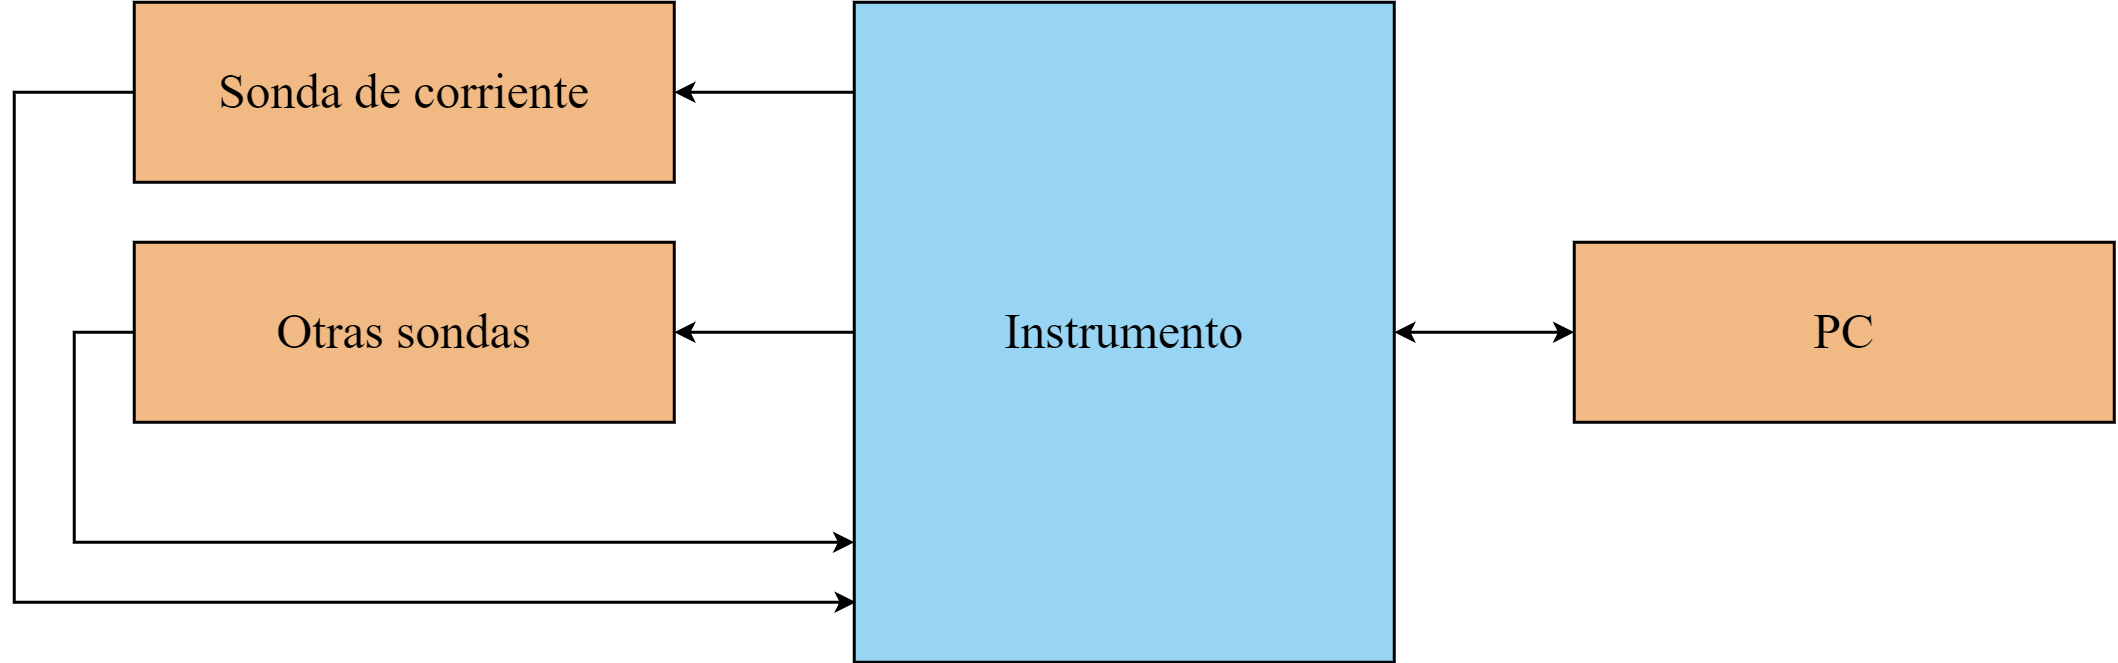
\includegraphics[width=0.9\textwidth]{diagrams/bloques-general.png}
    \caption{Diagrama en bloques general del dispositivo}
    \label{fig:bloques-general}
  \end{figure}

  Las corrientes generadas por el instrumento deberán poder ser medidas por las sondas externas y se deberá incorporar puertos que permitan conectarlas al mismo.

  %% ----------------------------------------------------------------
  \subsection{Características de los usuarios}
  %% ----------------------------------------------------------------
  Los usuarios del dispositivo serán aquellos estudiantes o investigadores que trabajen con sondas de corrientes y necesiten calibrarlas o caracterizarlas. Los mismos deberán tener conocimientos de electrónica para utilizar el instrumento.

  %% ----------------------------------------------------------------
  \subsection{Restricciones}
  %% ----------------------------------------------------------------
  \begin{table}[H]
    \centering
    \begin{tabulary}{0.8\textwidth}{|C|L|}
    \hline
      \rowcolor[HTML]{C0C0C0}
      Restricción & \multicolumn{1}{c|}{\cellcolor[HTML]{C0C0C0}Explicación} \\ \hline
      Potencia de corriente & Los componentes a utilizar presentan un máximo de corriente posible de generar. Si se sobrepasara el mismo, se podría dañar irreversiblemente el equipo. Es así, que se le debe agregar protección por sobrecorriente al equipo. \\ \hline
      Interfaz gráfica para el control del sistema & El sistema requiere una interfaz gráfica accesible a través de una computadora para su control. \\ \hline
      Lenguaje de programación del microcontrolador & Los microcontroladores están limitados a utilizar como lenguaje de programación el lenguaje C o C++. \\ \hline
    \end{tabulary}
  \end{table}


  %% ----------------------------------------------------------------
  \section{Requerimientos funcionales}
  %% ----------------------------------------------------------------

  %% ----------------------------------------------------------------
  \subsection{RF01: Generación y adquisición de corriente}
  %% ----------------------------------------------------------------
  El instrumento deberá generar corriente alterna senoidal, así como otras formas de onda que elija el usuario. Deberá también adquirir esa corriente generada para así realizar un control a lazo cerrado de la misma.

  Se permitirá que sondas de corriente externas midan esa corriente generada y se conecten al dispositivo, que adquirirá esas mediciones para su posterior caracterización y/o calibración.


  %% ----------------------------------------------------------------
  \subsection{RF02: Sistema de control gráfico y gestión de ensayos}
  %% ----------------------------------------------------------------
  El dispositivo deberá ser capaz de conectarse a una PC que utilice el sistema operativo Windows. En la misma correrá una interfaz gráfica que permitirá darle instrucciones al instrumento, así como también reportar información proveniente del mismo.

  Este sistema deberá ser capaz de realizar ensayos automatizados. El usuario introducirá los parámetros necesarios del ensayo en la interfaz gráfica en la PC, para que al finalizar el mismo, genere un reporte de las sondas conectadas.


%% ----------------------------------------------------------------
\section{Requerimientos no funcionales}
%% ----------------------------------------------------------------

  %% ----------------------------------------------------------------
  \subsection{RNF01: Generación de informes en PDF o JPG}
  %% ----------------------------------------------------------------
  Los informes mostrados en la interfaz gráfica deberán poder ser guardados en formato PDF o JPG, para su posterior uso.

  %% ----------------------------------------------------------------
  \subsection{RNF02: Guardado de datos en formato CSV}
  %% ----------------------------------------------------------------
  Los datos generados en los reportes deberán poder ser guardados en formato CSV. Esto permitirá al usuario acceder a los datos ``crudos'' y realizar así, en caso de necesitarlo, un procesado adicional.

  %% ----------------------------------------------------------------
  \subsection{RNF03: Registro de eventos}
  %% ----------------------------------------------------------------
  La interfaz gráfica deberá tener implementado un registro de eventos o \emph{logging} que permita al usuario obtener información de los distintos sucesos que ocurran en el dispositivo.

\end{document}
